\chapter{Design and implementation}

This chapter will describe details of implementation and design of my test application, frameworks that was used, adaptation for that frameworks and actual CellBE proting process details.

\section{Used frameworks}

\par
I decided to take ITK (\url{www.itk.org}) implementation of level set method as a base. So i have to get familiar with this huge project. It contains many algorithm implementations as well as necessary infrastructure content such as loading and saving variety of formats. Base concept of this project is pipeline and filters. To get some work done pipeline has to be build from filters. Filter is entity that represent an algorithm. When pipline is created the last filter is started. Starting event then propagate towards the beginnig of the pipeline where actual computation starts. Output from one filter is input of the following. Filters thus create a building blocks for some more complicated method.

\par
After some first test with example implementation I wrote my own testing application that was able load image, run the level set filter and save the results. I found out some reasonable parameter values with this. Because this pilot (originally with code name 'pok') application was controled via bash scripts that is not much easy nor user friendly and because there is no way how to visualize the results I decided to use another framework to overcome this problems, the Medv4D project (\url{http://cgg.mff.cuni.cz/trac/medv4d}).

\par
This project that was originally started as sofware project and that I was participating is basically framework for creation of medical applications. Its purpose is to simplify process of GUI creation as well as actual computation model design. Instead the programmer should focus on actual problem solution. Basic building block is also a filter. The filter can be merged into pipeline just like in ITK. But the Medv4D filters are more lowlevel and thus faster that ITK ones (speed was another goal of the framework). The pipeline then offer some implicit locking of dataset parts to allow parallel computation.

\section{Incorporation into Medv4D framework}

\par
The most convinient way how to incorporate ITK pipeline that is to be run on CellBE seemed client/server architecture. So the part of the application that has to be run on CellBE is server. While client part loads initial data (and saves the results), visualize the results and act as GUI with controls for parameter tunnig. Whole process can be described this way: client loads the input data sends them to server and waits for the results. As soon as the results is read it is visualized. Then the result can be saved or sent to server again for computation with another parameters. See Figure \ref{fg:computationProcess} showing how the application with code name 'RemoteCellLevelSet' works.

\begin{figure}
    \centering
    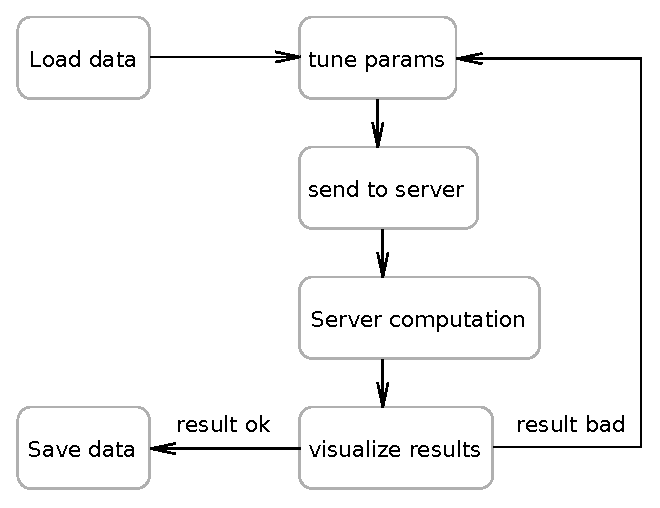
\includegraphics[width=14cm]{data/computationProcess.eps}
    \caption[RemoteCellLevelSet application computation process]{Client acts like GUI for the server side that performs actual computation}
    \label{fg:computationProcess}
\end{figure}

\par
There was some neccessary goals for incorporate 'pok' into Medv4D framework:
\begin{enumerate}
  \item{ITK integration}
  \par
  This is performed by wrapper Medv4D filter that is connected into Medv4D pipeline. Within this filter are two ITK images that serves as input and output for inner ITK pipeline. Actual data of this ITK images point to data of containing Medv4D wrapper filter (see Figure \ref{fg:ITKWrapping} for details).

  \item{Remote computing infrastructure}
  \par
  Infrastructure for sending commands to server along with data or parameter values as well recieving response messages along with resulting data had to be implemented into Medv4D. It lead into designing whole new library of Medv4D called remote computing. On client side it is representing by a remote filter that encapsulate whole infrastructure necessary for sending part of pipeline that the filter represents to server as well as result handling. Server side had to be designed completely as a whole.
\end{enumerate}

\begin{figure}
    \centering
    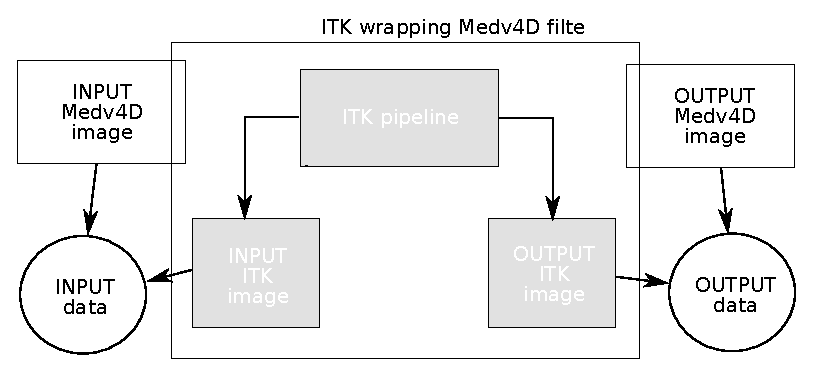
\includegraphics[width=12cm]{data/ITKFilter.eps}
    \caption[ITK wrapper Medv4D filter]{Basic elements are the two ITK images whose data are actually Medv4D images' data}
    \label{fg:ITKWrapping}
\end{figure}

\subsection{Client remote computing (RC) part}

As mentioned above base element of client RC part is remote filter. It implements actual command sending and result receiving functionality. It is derived from pipeline Medv4D filter so it can be added into pipeline. This part of pipeline that the remote filter represents thus run on remote server. Listing of commands that the remote filter issue to the server:
\begin{enumerate}
  \item{CREATE}
  \par
  This command is create request. It idetify the type of the filter that the remote filter represents and that shoult be instantiated on the server. Server parses the command message and instantiate appropriate filter along with whole pipeline (remote pipeline).

  \item{DATASET}
  \par
  Tells the server to read actual dataset that the computation will be performed on. The dataset is parameter of the command.

  \item{EXEC}
  Is request for actual execution of the remote pipeline. But before that parameter of this command which are filter parameter values should be parsed. After the parsing and association of filter parameters with actual filter is the remote pipeline executed.
\end{enumerate}

\par
Purpose of the commands is to divide actual execution into stages and thus to define a state of remote execution. This is because when actual dataset is send to server it would be worthless to send it again when user wants to execute remote pipeline again only with different parameters. So commands allow this because remote pipeline has state telling 'data already recieved now waiting for EXEC command as many times as wanted without no more input data transmission'.
\par
The Medv4D pipeline filter defines also some stages that the behaviour of remote filter benefits. That is there are method that is called only when input data chages (PrepareOutputDataset). This is perfect place to send DATASET command to server. Because this is called only on input data change thus DATASET command will be issued on input data change as well.
\par
CREATE command is sent in constructor of remote filter thus when pipeline is constructed which is usually at program startup. And EXEC command is then send within function that is called when pipeline is executed and that shoud perform actual computation (ProcessImage). Whole cycle shows Figure \ref{fg:RCClientCycle}.

\begin{figure}
    \centering
    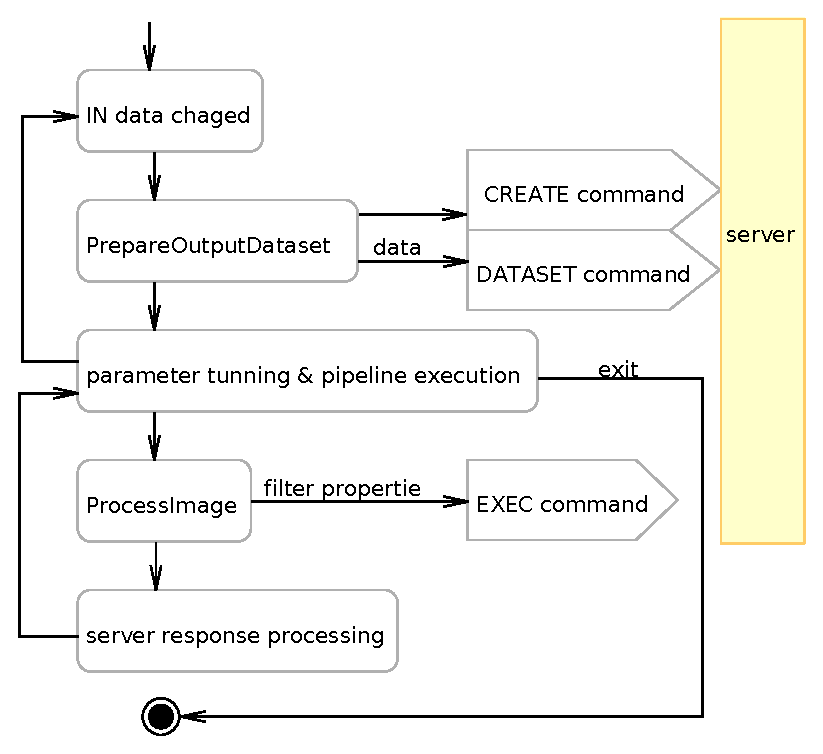
\includegraphics[width=12cm]{data/RCClientCycle.eps}
    \caption[Remote Medv4D filter]{Shows three basic states of remote filter and when particular command are sent to server.}
    \label{fg:RCClientCycle}
\end{figure}

Server response can be either OK or FIALED. In case of OK resulting dataset is received in contrast to FAILED case when no dataset is expected.

\subsection{Server RC part}

Server part is counter part of client one so the designe reflects it. Goal of server is to sit and wait for incomming connection. One connection means one session of computation. Currently only one session at a time is held. In context of a session command from client are parsed and appropriate actions performed (see Figure \ref{fg:RCServerCycle}).

\begin{figure}
    \centering
    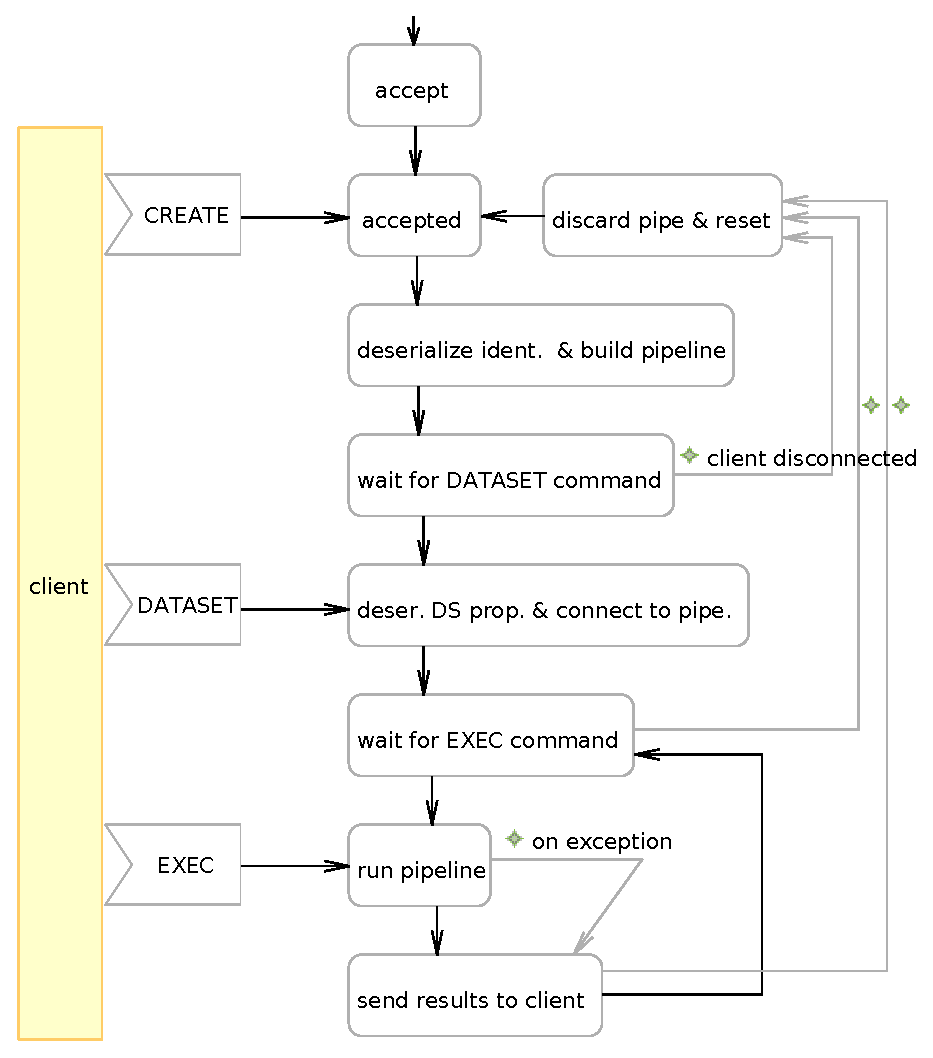
\includegraphics[width=12cm]{data/RCServerCycle.eps}
    \caption[MedV4D server cycle]{}
    \label{fg:RCServerCycle}
\end{figure}

Like in every client/setver application some kind of stubs are needed. In context of RemoteCellLevelSet application client/server pair the meaning of the stubs are serialization and deserialization methodes. Goal of the methodes is ensure that data that the client sends will be recieved in exactly the same order and data types. Good example is the CREATE request. In this request identifier of remote filter are send along with template parameters identifiers (because filter classes are templated). In case of mismatch of that identifiers completely different class would be instantiated. Hierarchy of virtual methodes on dataset classes defines interface for such stubs. Interface on remote filter properties class hierarchy does the same for remote filter.

Another issue is endianess. Endianess identifier is sent along with every command. On the other side is made decision if byte swapping should be performed. This allows to perform byte swapping only when it is really needed.

Currently only remote filter is implemented, the level set segmentation. But other filters can be easily added by appending one switch branch in remoteFilterFactory.cpp source. The level set segmentation filter is implemented as successor of ITK filter that contains appropriate ITK pipeline within. This pipeline is most interresting part related to this work so further content will be about it.

\section{Level set segmentation pipeline}

This pipeline contains three ITK filters.
\begin{enumerate}
  \item{fast marching filter}
  \par
  Is responsible for computation of initial level set. Parameters of this filter are point $\vec{x}$ in dataset and distance $d$. Output is then level set that corresponds to ball shaped level set with radius $d$.

  \item{level set segmentation filter (LS Filter)}
  \par
  Performs actual level set segmentation method. Parameters of this filter are threshold interval (thresholding level set segmentation),  maximal count of algorithm iterations (explained later), curvature and speed scaling (explained above).

  \item{binary thresholding filter}
  \par
  Purpose of this filter is extract resulting object from level set. It is thresholding that select pixels with values less that zero that corresponds to inner part of the resulting level set.
\end{enumerate}

I have chosen ITK sparse field method implementation as a starting point. This implementation uses linked lists to represent the sparse field layers. Actual algorithm as described higher (\ref{alg:sparseFileld}) is implemented in several classes. Due to mapping the algorithm to CellBE radical changes in code would be necessary even in ITK code. So i decided to rebuild appropriate part of ITK class hierarchy responsible for the sparse field level set computation (LS hierarchy) to create actual LS Filter. I borrowed some part of original code and inherited my classes from classes close to finite difference solver (FDS) class, see Figure\ref{fg:originalHierarchy}. In the original LS hierarchy are actually two hierarchies of classes. One represents the filter that performs level set evolution algorithm, filter hierarchy and the other finite \emph{difference function} that computes the finite differences (the upwind scheme), function hierarchy.
 
In function hierarchy the base is FiniteDifferenceFunction that computes the 'upwind scheme' with assistance of virtual methodes, that are implemented in successors. Successors are LevelSetFunction that provides curvature term computation methodes, SegmentationLevelSetFunction provides speed image computation based on speed image that computes ThresholdSegmentationLevelSetFunction. 

//TODO zeptat se jak se popisuje algoritmus ...
In filter hierarchy everything starts with FiniteDifferenceImageFilter that computes main loop of level set calculation (see step 1 in \ref{alg:sparseFileld}). Virtual methodes of its successors are used (just like in function hierarchy) to implement sub steps. Successor is the SparseFieldLevelSetImageFilter providing implementation of Step 1a , the \emph{update calculation} function and other steps by \emph{apply update calculation} function. Next successors, SegmentationLevelSetImageFilter and ThresholdSegmentationLevelSetImageFilter only manage \emph{difference function} in their own manner. In case ThresholdSegmentationLevelSetImageFilter manages speed function as described in \ref{eq:speedFunction}. It preallocates another image for precalculation of the speed function. This another image is another notable amount of memory that can not be accepted for my purpose (PS3 that I have available has only 256MB including operating system). This precalculation was one reason of inheritance from classes close to FDS. Speed function is calculated every time it is needed without any precalculations in my approach. This approach could be even better for CellBE streaming nature. The second reason was to simplify the structure of hierarchy and some code cleen-up and refactorization.

\begin{figure}
    \centering
    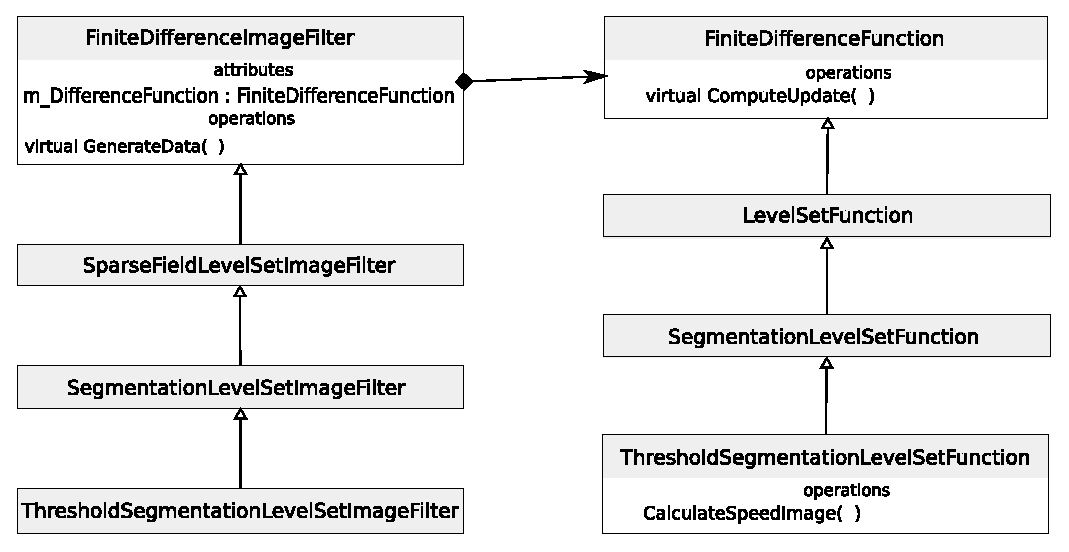
\includegraphics[width=15cm]{data/originalHierarchy.eps}
    \caption[Original ITK thresholding level set filter class hierarchy]{Illustrates the FiniteDifferenceFunction hierarchy and the FiniteDifferenceImageFilter hierarchy and their relationship}
    \label{fg:originalHierarchy}
\end{figure}

Result of this changes is my own filter (ThreshSegLevelSetFilter) that omits all unnecessary part of original LS hierarchy, uses reasonable parts of the original ITK level set segmentation filter and is ready to be ported for CellBE (see Figure\ref{fg:resultingFilter}). In the function hierarchy stayed only the base class that the resulting ThresholdLevelSetFunc class is derived. This new class does the same job as original LS function hierachy but in manner closer to streaming architecture (the prealocation of the speed image is ommited). The computation of particular up-wind scheme terms was separated into stand alone classes for more code readability and modularity. The filter hierarchy was shortend and begins already in SparseFieldLevelSetImageFilter. All the successors in orginal hierarchy was ommited since they did anything reasonable. Some function implementation from the SparseFieldLevelSetImageFilter was borrowed into the new ThreshSegLevelSetFilter to be tuned for CellBE.

\begin{figure}
    \centering
    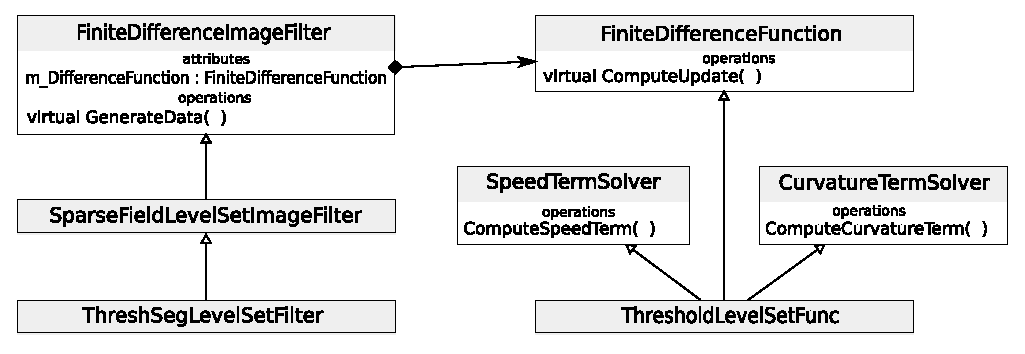
\includegraphics[width=15cm]{data/resultingFilter.eps}
    \caption[Resulting level set filter ready to be ported to CellBE]{Show result of original LS hierarchy rebuilding. Some unnecessary parts was ommited to clean-up the code and to change behaviour towards straming architecture as well as term computation was separated into supporting classes for modularity}
    \label{fg:resultingFilter}
\end{figure}

\section{Actual porting process}

Server application with the thresholding level set filter within was build and then profiled. As the first step of the porting process.

//TODO tabulka s vysledky

\chapter{Results}
Tabulka:::
\begin{center}
\begin{tabular}{|l|c|p{3.5in}|}
\hline
\multicolumn{3}{|c|}{Nazev tabulky}\\ 
\hline cell 1&cell 2&cell 3\\&todle bude pod cell 2, protoze to je mezi dvema'\&' &\\ 
\hline Big Basin&1.5&Very nice overnight to Berry Creek Falls from
either Headquarters or ocean side.\\ 
\hline Sunol&1&Technicolor green in the spring. Watch out for the cows.\\ 
\hline Henry Coe&1.5&Large wilderness nearby suitable for multi-day treks.\\ 
\hline
\end{tabular}
\end{center}

The profiling shows that the most time consuming parts of the program is not the difference solving in update calculation step but the update application step. The original idea was to offload only the difference solving within the update calculation step which is performed on $$3^3$$ voxel matrix and calculated independently of the others which makes this job perfectly suited for offloading to SPE. But the time taken for computation of this part is only the fragment of the whole. This is the reason for another changes to the ITK class hierarchy and new level set filter design. Actualy the whole program is rebuild and from original ITK class hierarchy last nothing. Everything replaced by the ThreshSegLevelSetFilter in conjuction with my version of original FinititeDifferenceImageFilter (FDIF) where the main loop of the algorithm as well as stopping conditions resides. The reason of replacing even the FDIF is that it suppose usage of a difference function. It had appropriate virtual methodes that expects it. But in the new design the difference function will be offloaded as well so it was taken out completely through the MyFDIF.

Further figure shows structure of the new design

\begin{figure}
    \centering
    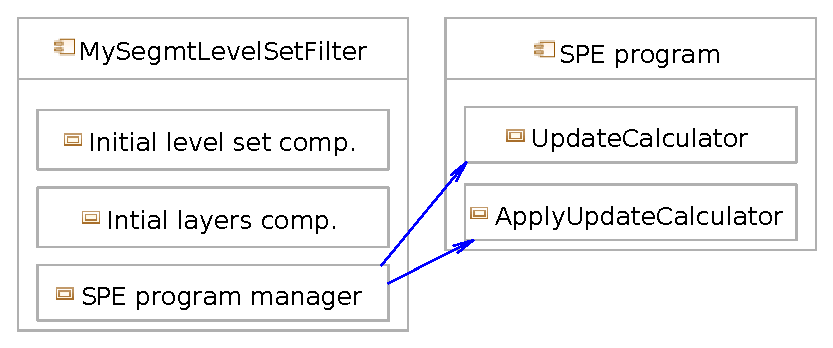
\includegraphics[width=15cm]{data/newDesign.eps}
    \caption[Diagram of new design components]{//TODO}
    \label{fg:newDesign}
\end{figure}

On the figure \ref{fg:newDesign} can be noticed that almost whole original ITK pipeline is offloaded to SPE. Only initialization routines are left to PPE. This lead to create the SPE program manager that will manage computations on SPEs. It is responsible for SPE thread initialization and run, and SPEs synchronization.

SPE part consists of two main parts. The UpdateCalculator, performing \emph{apply update calculation} and ApplyUpdateCalculator, performng \emph{apply update calculation}.

//popsat algoritmus vic do hloubky, co se kde produkuje
//jak se to bude prenaset mezu SPU a PPU

//analogie s pracovnikama a managerama

//TODO popsat kde objekty ziji
//popsat jednotlive tooly a vztah k Cell featuram

//popsat process jak celou dobu pro PC a jenom casti, ktery spolu komunikujou (tooly) jsou simulovany memcp()